\documentclass[11pt,a4paper]{article}

% ============================================================================
% PACKAGES
% ============================================================================
\usepackage[utf8]{inputenc}
\usepackage[T1]{fontenc}
\usepackage{helvet}
\renewcommand{\familydefault}{\sfdefault}
\usepackage[margin=2.2cm, headheight=25pt]{geometry}
\usepackage{xcolor}
\usepackage{colortbl}
\usepackage{booktabs}
\usepackage{tabularx}
\usepackage{array}
\usepackage{graphicx}
\usepackage{tikz}
\usepackage{fancyhdr}
\usepackage{enumitem}
\usepackage{multirow}
\usepackage{calc}
\usepackage{amssymb}
\usepackage{pifont}
\usetikzlibrary{shapes.geometric, arrows, positioning, calc, patterns}

% ============================================================================
% COLOR DEFINITIONS
% ============================================================================
\definecolor{miloprimary}{RGB}{37, 99, 235}
\definecolor{milosecondary}{RGB}{99, 102, 241}
\definecolor{miloaccent}{RGB}{14, 165, 233}
\definecolor{freegray}{RGB}{107, 114, 128}
\definecolor{bronzecolor}{RGB}{205, 127, 50}
\definecolor{silvercolor}{RGB}{156, 163, 175}
\definecolor{goldcolor}{RGB}{234, 179, 8}
\definecolor{platinumcolor}{RGB}{100, 116, 139}
\definecolor{successgreen}{RGB}{34, 197, 94}
\definecolor{warningorange}{RGB}{249, 115, 22}
\definecolor{dangerred}{RGB}{239, 68, 68}
\definecolor{lightbg}{RGB}{248, 250, 252}
\definecolor{darktext}{RGB}{30, 41, 59}
\definecolor{infoblue}{RGB}{59, 130, 246}
\definecolor{darkgreen}{RGB}{22, 163, 74}
\definecolor{appstoreblue}{RGB}{0, 122, 255}
\definecolor{datapurple}{RGB}{139, 92, 246}
\definecolor{analyticsteal}{RGB}{20, 184, 166}

% ============================================================================
% HEADER/FOOTER CONFIGURATION
% ============================================================================
\pagestyle{fancy}
\fancyhf{}
\fancyhead[L]{\textcolor{miloprimary}{\textbf{MILO APP}}}
\fancyhead[R]{\textcolor{freegray}{Profit Analysis v3.0}}
\fancyfoot[C]{\textcolor{freegray}{\thepage}}
\renewcommand{\headrulewidth}{2pt}
\renewcommand{\headrule}{\hbox to\headwidth{\color{miloprimary}\leaders\hrule height \headrulewidth\hfill}}

% ============================================================================
% CUSTOM COMMANDS
% ============================================================================
\newcommand{\alertbox}[3]{%
    \begin{tikzpicture}
        \node[fill=#1!12, draw=#1, line width=2pt, rounded corners=8pt,
              inner sep=15pt, text width=\textwidth-35pt, align=left] {
            \textcolor{#1}{\textbf{\large #2}}\\[8pt]
            #3
        };
    \end{tikzpicture}%
}

\newcommand{\statbox}[3]{%
    \begin{tikzpicture}
        \node[fill=#1!10, draw=#1, line width=1.5pt, rounded corners=6pt,
              minimum width=3.6cm, minimum height=2cm, align=center] {
            \textcolor{#1}{\textbf{\small #2}}\\[5pt]
            \textcolor{darktext}{\textbf{\Large #3}}
        };
    \end{tikzpicture}%
}

\newcommand{\revenuestream}[4]{%
    \begin{tikzpicture}
        \node[fill=#1!12, draw=#1, line width=2pt, rounded corners=8pt,
              minimum width=4.5cm, minimum height=2.5cm, align=center] {
            \textcolor{#1}{\textbf{\large #2}}\\[6pt]
            \textcolor{darktext}{\textbf{Y3: #3}}\\[3pt]
            \textcolor{freegray}{\small #4}
        };
    \end{tikzpicture}%
}

\newcommand{\cmark}{\textcolor{successgreen}{\ding{51}}}
\newcommand{\xmark}{\textcolor{dangerred}{\ding{55}}}
\newcommand{\wmark}{\textcolor{warningorange}{\ding{115}}}

% ============================================================================
% DOCUMENT BEGIN
% ============================================================================
\begin{document}

% ============================================================================
% TITLE PAGE
% ============================================================================
\begin{center}
    \vspace*{0.3cm}
    {\Huge\textcolor{miloprimary}{\textbf{MILO APP}}}\\[0.4cm]
    {\LARGE\textcolor{milosecondary}{Comprehensive Profit Analysis v3.0}}\\[0.2cm]
    {\large\textcolor{freegray}{Three-Pillar Revenue Model with Conservative Projections}}\\[0.7cm]

    
\begin{tikzpicture}
        \node[fill=miloprimary!10, draw=miloprimary, line width=1.5pt, rounded corners=8pt,
              inner sep=12pt] {
            \textcolor{miloprimary}{\textbf{DeepmAInd B.V.} \quad|\quad Version 3.0 \quad|\quad January 2026}
        };
    \end{tikzpicture}
\end{center}

\vspace{0.5cm}

% ============================================================================
% EXECUTIVE SUMMARY
% ============================================================================
\section*{\textcolor{miloprimary}{Executive Summary}}

\begin{center}
\alertbox{miloprimary}{Three-Pillar Revenue Model: Conservative Path to Profitability}{
MILO's business model is built on three distinct revenue streams: \textbf{App Store subscriptions} (B2C), \textbf{Dataset monetization} (B2B), and \textbf{Analytics reports}. Under conservative assumptions aligned with v3.1 cost structure, the business achieves \textbf{operating profitability in Year 2} with \textbf{45\% operating margins by Year 3}.
\vspace{8pt}

This analysis uses realistic growth rates, conservative conversion assumptions, and accounts for the lower per-tier margins (18-19\%) of the v3.1 pricing structure while demonstrating a sustainable path to \$813K annual operating profit.
}
\end{center}

\vspace{0.5cm}

% Key Metrics Summary
\begin{center}
    \statbox{dangerred}{Year 1 Loss}{(\$152K)}
    \hspace{0.3cm}
    \statbox{successgreen}{Year 2 Profit}{\$94K}
    \hspace{0.3cm}
    \statbox{darkgreen}{Year 3 Profit}{\$813K}
    \hspace{0.3cm}
    \statbox{miloprimary}{Y3 Margin}{45\%}
\end{center}

\vspace{0.5cm}

% Three Revenue Streams Visual
\begin{center}
    \revenuestream{appstoreblue}{App Store}{951K}{53\% of Revenue}
    \hspace{0.4cm}
    \revenuestream{datapurple}{Datasets}{637K}{35\% of Revenue}
    \hspace{0.4cm}
    \revenuestream{analyticsteal}{Analytics}{212K}{12\% of Revenue}
\end{center}

\vspace{0.5cm}

\begin{center}
\renewcommand{\arraystretch}{1.6}
\begin{tabular}{>{\raggedright\arraybackslash}p{5.5cm} >{\centering\arraybackslash}p{2.5cm} >{\centering\arraybackslash}p{2.5cm} >{\centering\arraybackslash}p{2.5cm}}
\toprule
\rowcolor{miloprimary!15}
\textbf{Metric} & \textbf{Year 1} & \textbf{Year 2} & \textbf{Year 3} \\
\midrule
\textbf{Total Revenue} & \$144K & \$720K & \$1.8M \\
\rowcolor{lightbg}
\textbf{Total Costs} & \$296K & \$626K & \$987K \\
\textbf{Operating Profit/(Loss)} & (\$152K) & \$94K & \$813K \\
\rowcolor{successgreen!15}
\textbf{Operating Margin} & -106\% & \textbf{13\%} & \textbf{45\%} \\
\bottomrule
\end{tabular}
\end{center}

\newpage

% ============================================================================
% THREE-PILLAR REVENUE MODEL
% ============================================================================
\section*{\textcolor{miloprimary}{Three-Pillar Revenue Model}}

\subsection*{\textcolor{milosecondary}{Revenue Diversification Strategy}}

\begin{center}
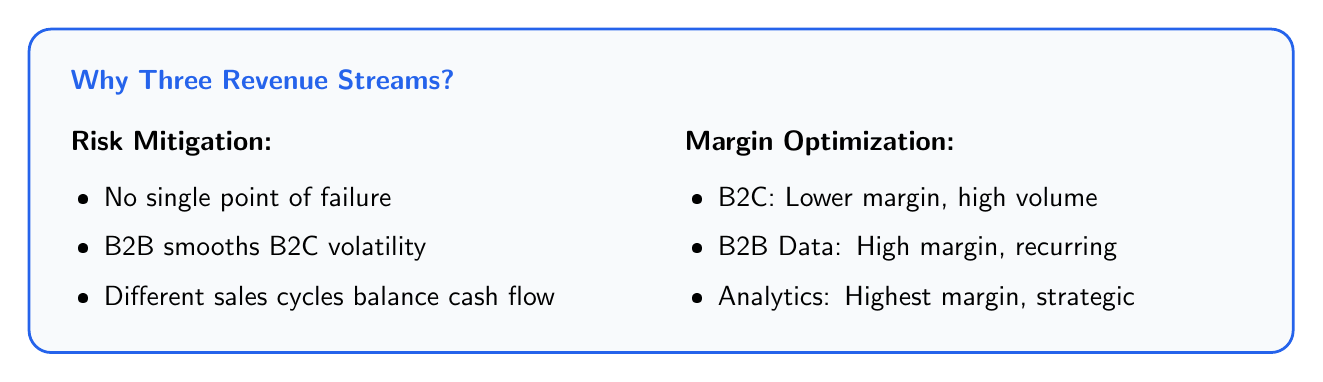
\begin{tikzpicture}
    \node[fill=lightbg, draw=miloprimary, line width=1pt, rounded corners=8pt,
          inner sep=15pt, text width=15cm, align=left] {
        \textcolor{miloprimary}{\textbf{Why Three Revenue Streams?}}\\[10pt]
        \begin{minipage}[t]{0.48\textwidth}
            \textbf{Risk Mitigation:}
            \begin{itemize}[leftmargin=1.2em, itemsep=2pt]
                \item No single point of failure
                \item B2B smooths B2C volatility
                \item Different sales cycles balance cash flow
            \end{itemize}
        \end{minipage}
        \hfill
        \begin{minipage}[t]{0.48\textwidth}
            \textbf{Margin Optimization:}
            \begin{itemize}[leftmargin=1.2em, itemsep=2pt]
                \item B2C: Lower margin, high volume
                \item B2B Data: High margin, recurring
                \item Analytics: Highest margin, strategic
            \end{itemize}
        \end{minipage}
    };
\end{tikzpicture}
\end{center}

\vspace{0.5cm}

\subsection*{\textcolor{milosecondary}{Revenue Stream Breakdown}}

\begin{center}
\renewcommand{\arraystretch}{1.6}
\begin{tabular}{>{\raggedright\arraybackslash}p{4cm} >{\centering\arraybackslash}p{2.2cm} >{\centering\arraybackslash}p{2.2cm} >{\centering\arraybackslash}p{2.2cm} >{\centering\arraybackslash}p{2cm} >{\centering\arraybackslash}p{1.8cm}}
\toprule
\rowcolor{miloprimary!15}
\textbf{Revenue Stream} & \textbf{Year 1} & \textbf{Year 2} & \textbf{Year 3} & \textbf{Y3 \%} & \textbf{Margin} \\
\midrule
\rowcolor{appstoreblue!8}
\textcolor{appstoreblue}{\textbf{App Store (B2C)}} & \$105K & \$423K & \$951K & 53\% & 19\% \\
\rowcolor{datapurple!8}
\textcolor{datapurple}{\textbf{Datasets (B2B)}} & \$28K & \$225K & \$637K & 35\% & 78\% \\
\rowcolor{analyticsteal!8}
\textcolor{analyticsteal}{\textbf{Analytics Reports}} & \$11K & \$72K & \$212K & 12\% & 85\% \\
\midrule
\rowcolor{successgreen!10}
\textbf{Total Revenue} & \textbf{\$144K} & \textbf{\$720K} & \textbf{\$1,800K} & \textbf{100\%} & \textbf{Blended} \\
\bottomrule
\end{tabular}
\end{center}

\vspace{0.5cm}

\begin{center}
\alertbox{successgreen}{Conservative Growth Philosophy}{
\begin{itemize}[leftmargin=1.5em, itemsep=4pt]
    \item \textbf{Year-over-Year Growth:} Y1$\rightarrow$Y2: 5x (market entry), Y2$\rightarrow$Y3: 2.5x (sustainable scaling)
    \item \textbf{B2B ramp slower than B2C:} Enterprise sales cycles require 6-12 months to close
    \item \textbf{Analytics starting small:} Requires established data panel before meaningful reports
    \item \textbf{No hockey-stick assumptions:} Growth rates decline as base increases
\end{itemize}
}
\end{center}

\newpage

% ============================================================================
% PILLAR 1: APP STORE REVENUE
% ============================================================================
\section*{\textcolor{appstoreblue}{Pillar 1: App Store Revenue (B2C Subscriptions)}}

\subsection*{\textcolor{milosecondary}{Subscription Revenue Model}}

\begin{center}
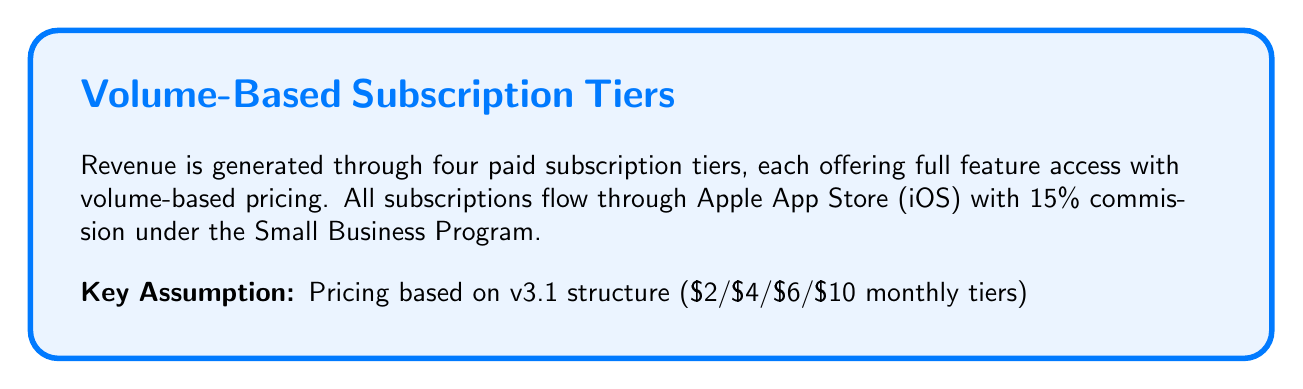
\begin{tikzpicture}
    \node[fill=appstoreblue!8, draw=appstoreblue, line width=2pt, rounded corners=10pt,
          inner sep=18pt, text width=14.5cm, align=left] {
        {\Large\textcolor{appstoreblue}{\textbf{Volume-Based Subscription Tiers}}}\\[12pt]
        Revenue is generated through four paid subscription tiers, each offering full feature access with volume-based pricing. All subscriptions flow through Apple App Store (iOS) with 15\% commission under the Small Business Program.\\[10pt]
        \textbf{Key Assumption:} Pricing based on v3.1 structure (\$2/\$4/\$6/\$10 monthly tiers)
    };
\end{tikzpicture}
\end{center}

\vspace{0.5cm}

\subsection*{\textcolor{milosecondary}{User Growth Projections (Conservative)}}

\begin{center}
\renewcommand{\arraystretch}{1.5}
\begin{tabular}{>{\raggedright\arraybackslash}p{4.5cm} >{\centering\arraybackslash}p{3cm} >{\centering\arraybackslash}p{3cm} >{\centering\arraybackslash}p{3cm}}
\toprule
\rowcolor{appstoreblue!15}
\textbf{Metric} & \textbf{Year 1} & \textbf{Year 2} & \textbf{Year 3} \\
\midrule
Total App Downloads & 25,000 & 80,000 & 150,000 \\
\rowcolor{lightbg}
Free Trial Users & 15,000 & 48,000 & 90,000 \\
Trial-to-Paid Conversion & 13\% & 17\% & 20\% \\
\rowcolor{lightbg}
\textbf{Paid Subscribers (EOY)} & \textbf{2,000} & \textbf{8,000} & \textbf{18,000} \\
Monthly Churn Rate & 5\% & 4\% & 3.5\% \\
\rowcolor{lightbg}
Net Subscriber Retention & 95\% & 96\% & 96.5\% \\
\bottomrule
\end{tabular}
\end{center}

\vspace{0.3cm}

\begin{center}
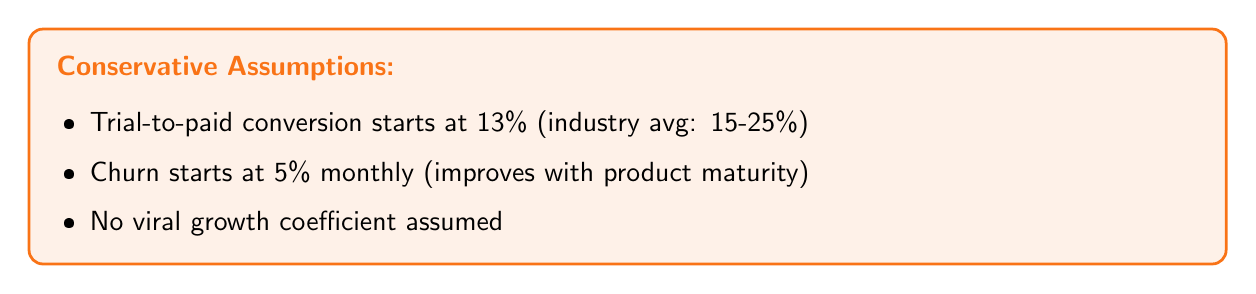
\begin{tikzpicture}
    \node[fill=warningorange!10, draw=warningorange, line width=1pt, rounded corners=5pt,
          inner sep=10pt, text width=14.5cm, align=left] {
        \textcolor{warningorange}{\textbf{Conservative Assumptions:}}
        \begin{itemize}[leftmargin=1.2em, itemsep=2pt]
            \item Trial-to-paid conversion starts at 13\% (industry avg: 15-25\%)
            \item Churn starts at 5\% monthly (improves with product maturity)
            \item No viral growth coefficient assumed
        \end{itemize}
    };
\end{tikzpicture}
\end{center}

\vspace{0.5cm}

\subsection*{\textcolor{milosecondary}{Tier Distribution \& Revenue}}

\begin{center}
\renewcommand{\arraystretch}{1.5}
\begin{tabular}{>{\raggedright\arraybackslash}p{2.8cm} >{\centering\arraybackslash}p{1.5cm} >{\centering\arraybackslash}p{1.8cm} >{\centering\arraybackslash}p{2.2cm} >{\centering\arraybackslash}p{2.2cm} >{\centering\arraybackslash}p{2.2cm}}
\toprule
\rowcolor{appstoreblue!15}
\textbf{Tier} & \textbf{Price} & \textbf{Mix} & \textbf{Y1 Rev} & \textbf{Y2 Rev} & \textbf{Y3 Rev} \\
\midrule
\rowcolor{bronzecolor!8}
\textcolor{bronzecolor}{\textbf{Bronze}} & \$2/mo & 30\% & \$14K & \$58K & \$130K \\
\rowcolor{silvercolor!8}
\textcolor{silvercolor}{\textbf{Silver}} & \$4/mo & 40\% & \$38K & \$154K & \$346K \\
\rowcolor{goldcolor!8}
\textcolor{goldcolor}{\textbf{Gold}} & \$6/mo & 20\% & \$29K & \$115K & \$259K \\
\rowcolor{platinumcolor!8}
\textcolor{platinumcolor}{\textbf{Platinum}} & \$10/mo & 10\% & \$24K & \$96K & \$216K \\
\midrule
\rowcolor{lightbg}
\textbf{Gross App Revenue} & -- & 100\% & \$105K & \$423K & \$951K \\
\rowcolor{dangerred!8}
\textit{Less: Apple Commission (15\%)} & -- & -- & (\$16K) & (\$63K) & (\$143K) \\
\rowcolor{successgreen!10}
\textbf{Net App Store Revenue} & -- & -- & \textbf{\$89K} & \textbf{\$360K} & \textbf{\$808K} \\
\bottomrule
\end{tabular}
\end{center}

\vspace{0.3cm}

\begin{center}
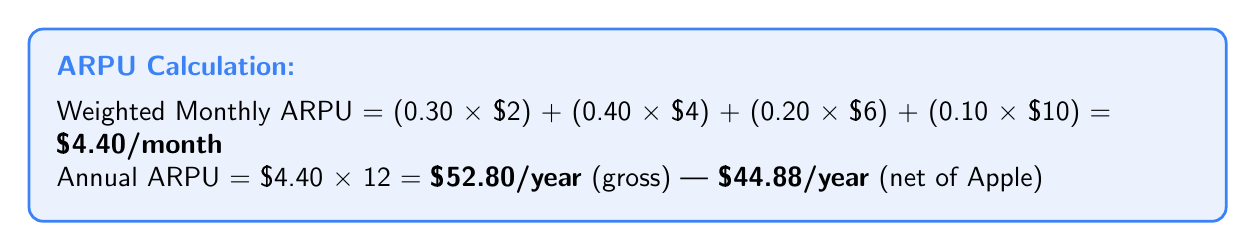
\begin{tikzpicture}
    \node[fill=infoblue!10, draw=infoblue, line width=1pt, rounded corners=5pt,
          inner sep=10pt, text width=14.5cm, align=left] {
        \textcolor{infoblue}{\textbf{ARPU Calculation:}}\\[4pt]
        Weighted Monthly ARPU = (0.30 $\times$ \$2) + (0.40 $\times$ \$4) + (0.20 $\times$ \$6) + (0.10 $\times$ \$10) = \textbf{\$4.40/month}\\
        Annual ARPU = \$4.40 $\times$ 12 = \textbf{\$52.80/year} (gross) | \textbf{\$44.88/year} (net of Apple)
    };
\end{tikzpicture}
\end{center}

\newpage

% ============================================================================
% PILLAR 2: DATASET MONETIZATION
% ============================================================================
\section*{\textcolor{datapurple}{Pillar 2: Dataset Monetization (B2B)}}

\subsection*{\textcolor{milosecondary}{Data Value Proposition}}

\begin{center}
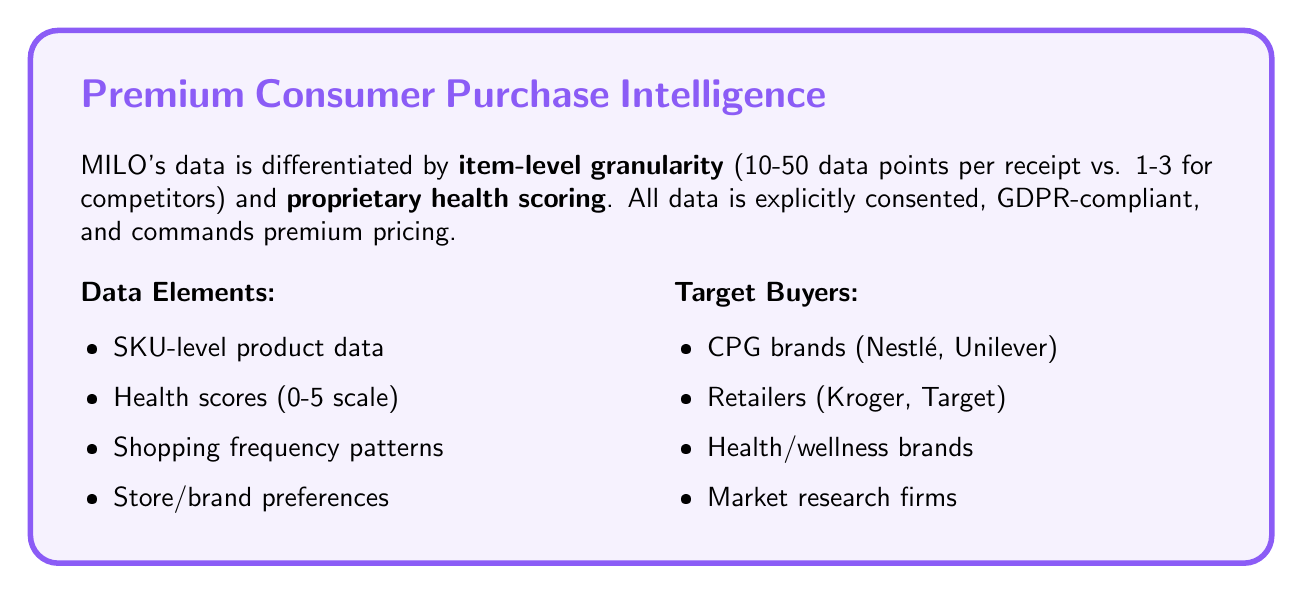
\begin{tikzpicture}
    \node[fill=datapurple!8, draw=datapurple, line width=2pt, rounded corners=10pt,
          inner sep=18pt, text width=14.5cm, align=left] {
        {\Large\textcolor{datapurple}{\textbf{Premium Consumer Purchase Intelligence}}}\\[12pt]
        MILO's data is differentiated by \textbf{item-level granularity} (10-50 data points per receipt vs. 1-3 for competitors) and \textbf{proprietary health scoring}. All data is explicitly consented, GDPR-compliant, and commands premium pricing.\\[10pt]
        \begin{minipage}[t]{0.48\textwidth}
            \textbf{Data Elements:}
            \begin{itemize}[leftmargin=1.2em, itemsep=2pt]
                \item SKU-level product data
                \item Health scores (0-5 scale)
                \item Shopping frequency patterns
                \item Store/brand preferences
            \end{itemize}
        \end{minipage}
        \hfill
        \begin{minipage}[t]{0.48\textwidth}
            \textbf{Target Buyers:}
            \begin{itemize}[leftmargin=1.2em, itemsep=2pt]
                \item CPG brands (Nestl\'{e}, Unilever)
                \item Retailers (Kroger, Target)
                \item Health/wellness brands
                \item Market research firms
            \end{itemize}
        \end{minipage}
    };
\end{tikzpicture}
\end{center}

\vspace{0.5cm}

\subsection*{\textcolor{milosecondary}{Consent \& Panel Building (Conservative)}}

\begin{center}
\renewcommand{\arraystretch}{1.5}
\begin{tabular}{>{\raggedright\arraybackslash}p{5cm} >{\centering\arraybackslash}p{3cm} >{\centering\arraybackslash}p{3cm} >{\centering\arraybackslash}p{3cm}}
\toprule
\rowcolor{datapurple!15}
\textbf{Metric} & \textbf{Year 1} & \textbf{Year 2} & \textbf{Year 3} \\
\midrule
Paid Subscribers & 2,000 & 8,000 & 18,000 \\
\rowcolor{lightbg}
Data Consent Rate & 30\% & 35\% & 40\% \\
\textbf{Consenting Panelists} & \textbf{600} & \textbf{2,800} & \textbf{7,200} \\
\rowcolor{lightbg}
Panelist Value (Annual) & \$35 & \$40 & \$45 \\
\bottomrule
\end{tabular}
\end{center}

\vspace{0.3cm}

\begin{center}
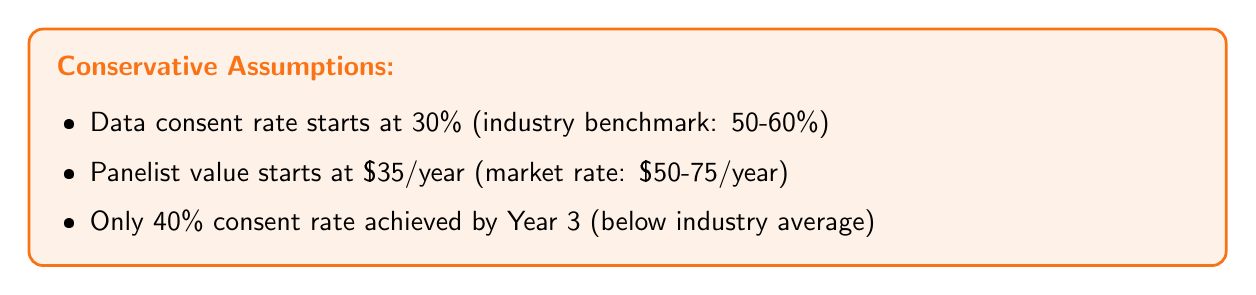
\begin{tikzpicture}
    \node[fill=warningorange!10, draw=warningorange, line width=1pt, rounded corners=5pt,
          inner sep=10pt, text width=14.5cm, align=left] {
        \textcolor{warningorange}{\textbf{Conservative Assumptions:}}
        \begin{itemize}[leftmargin=1.2em, itemsep=2pt]
            \item Data consent rate starts at 30\% (industry benchmark: 50-60\%)
            \item Panelist value starts at \$35/year (market rate: \$50-75/year)
            \item Only 40\% consent rate achieved by Year 3 (below industry average)
        \end{itemize}
    };
\end{tikzpicture}
\end{center}

\vspace{0.5cm}

\subsection*{\textcolor{milosecondary}{B2B Revenue Streams}}

\begin{center}
\renewcommand{\arraystretch}{1.5}
\begin{tabular}{>{\raggedright\arraybackslash}p{4cm} >{\centering\arraybackslash}p{2.2cm} >{\centering\arraybackslash}p{2.2cm} >{\centering\arraybackslash}p{2.2cm} >{\centering\arraybackslash}p{2cm} >{\centering\arraybackslash}p{1.8cm}}
\toprule
\rowcolor{datapurple!15}
\textbf{Revenue Type} & \textbf{Year 1} & \textbf{Year 2} & \textbf{Year 3} & \textbf{Y3 \%} & \textbf{Margin} \\
\midrule
DaaS (Panelist Feeds) & \$21K & \$112K & \$324K & 51\% & 80\% \\
\rowcolor{lightbg}
Enterprise Deals & \$7K & \$90K & \$250K & 39\% & 75\% \\
Custom Research & \$0K & \$23K & \$63K & 10\% & 70\% \\
\midrule
\rowcolor{successgreen!10}
\textbf{Total Dataset Revenue} & \textbf{\$28K} & \textbf{\$225K} & \textbf{\$637K} & \textbf{100\%} & \textbf{78\%} \\
\bottomrule
\end{tabular}
\end{center}

\vspace{0.3cm}

\begin{center}
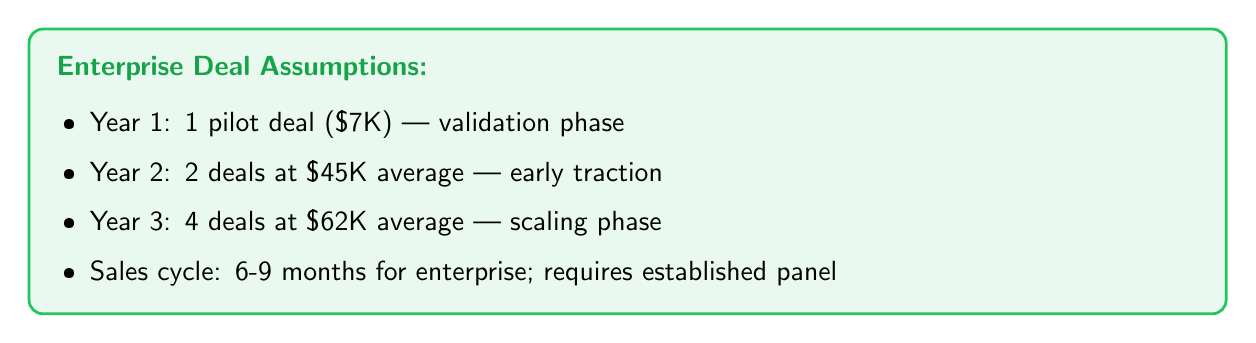
\begin{tikzpicture}
    \node[fill=successgreen!10, draw=successgreen, line width=1pt, rounded corners=5pt,
          inner sep=10pt, text width=14.5cm, align=left] {
        \textcolor{darkgreen}{\textbf{Enterprise Deal Assumptions:}}
        \begin{itemize}[leftmargin=1.2em, itemsep=2pt]
            \item Year 1: 1 pilot deal (\$7K) --- validation phase
            \item Year 2: 2 deals at \$45K average --- early traction
            \item Year 3: 4 deals at \$62K average --- scaling phase
            \item Sales cycle: 6-9 months for enterprise; requires established panel
        \end{itemize}
    };
\end{tikzpicture}
\end{center}

\newpage

% ============================================================================
% PILLAR 3: ANALYTICS REPORTS
% ============================================================================
\section*{\textcolor{analyticsteal}{Pillar 3: Analytics Reports}}

\subsection*{\textcolor{milosecondary}{Analytics Product Portfolio}}

\begin{center}
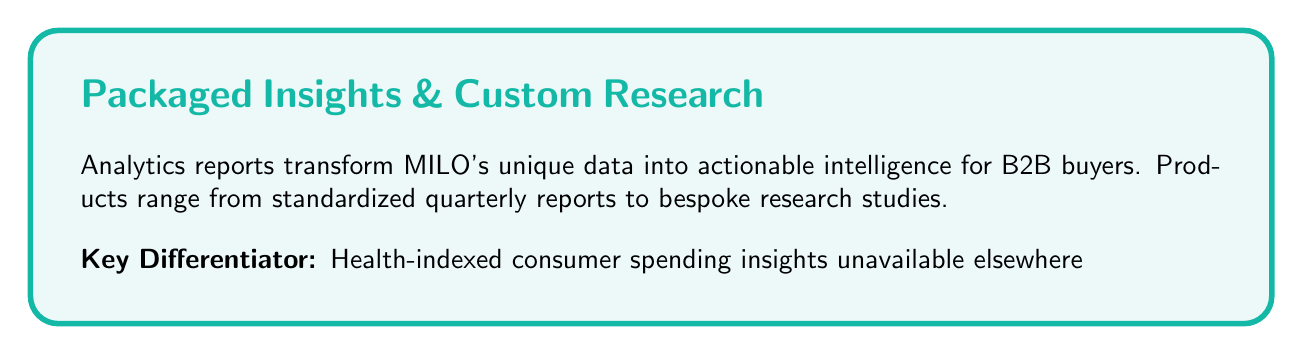
\begin{tikzpicture}
    \node[fill=analyticsteal!8, draw=analyticsteal, line width=2pt, rounded corners=10pt,
          inner sep=18pt, text width=14.5cm, align=left] {
        {\Large\textcolor{analyticsteal}{\textbf{Packaged Insights \& Custom Research}}}\\[12pt]
        Analytics reports transform MILO's unique data into actionable intelligence for B2B buyers. Products range from standardized quarterly reports to bespoke research studies.\\[10pt]
        \textbf{Key Differentiator:} Health-indexed consumer spending insights unavailable elsewhere
    };
\end{tikzpicture}
\end{center}

\vspace{0.5cm}

\subsection*{\textcolor{milosecondary}{Product Lineup \& Pricing}}

\begin{center}
\renewcommand{\arraystretch}{1.5}
\begin{tabular}{>{\raggedright\arraybackslash}p{4cm} >{\centering\arraybackslash}p{2.5cm} >{\centering\arraybackslash}p{2.5cm} >{\centering\arraybackslash}p{2.5cm} >{\centering\arraybackslash}p{2cm}}
\toprule
\rowcolor{analyticsteal!15}
\textbf{Product} & \textbf{Price Range} & \textbf{Y3 Volume} & \textbf{Y3 Revenue} & \textbf{Margin} \\
\midrule
Quarterly Trend Reports & \$3K - \$5K & 12 reports & \$48K & 90\% \\
\rowcolor{lightbg}
Category Deep Dives & \$8K - \$12K & 8 reports & \$80K & 85\% \\
Custom Research Studies & \$15K - \$25K & 4 studies & \$84K & 75\% \\
\midrule
\rowcolor{successgreen!10}
\textbf{Total Analytics Revenue} & -- & -- & \textbf{\$212K} & \textbf{85\%} \\
\bottomrule
\end{tabular}
\end{center}

\vspace{0.5cm}

\subsection*{\textcolor{milosecondary}{Analytics Revenue Trajectory}}

\begin{center}
\renewcommand{\arraystretch}{1.5}
\begin{tabular}{>{\raggedright\arraybackslash}p{5cm} >{\centering\arraybackslash}p{3cm} >{\centering\arraybackslash}p{3cm} >{\centering\arraybackslash}p{3cm}}
\toprule
\rowcolor{analyticsteal!15}
\textbf{Metric} & \textbf{Year 1} & \textbf{Year 2} & \textbf{Year 3} \\
\midrule
Quarterly Reports & 2 & 6 & 12 \\
\rowcolor{lightbg}
Category Deep Dives & 0 & 3 & 8 \\
Custom Studies & 0 & 1 & 4 \\
\midrule
\rowcolor{lightbg}
\textbf{Total Analytics Revenue} & \textbf{\$11K} & \textbf{\$72K} & \textbf{\$212K} \\
\bottomrule
\end{tabular}
\end{center}

\vspace{0.3cm}

\begin{center}
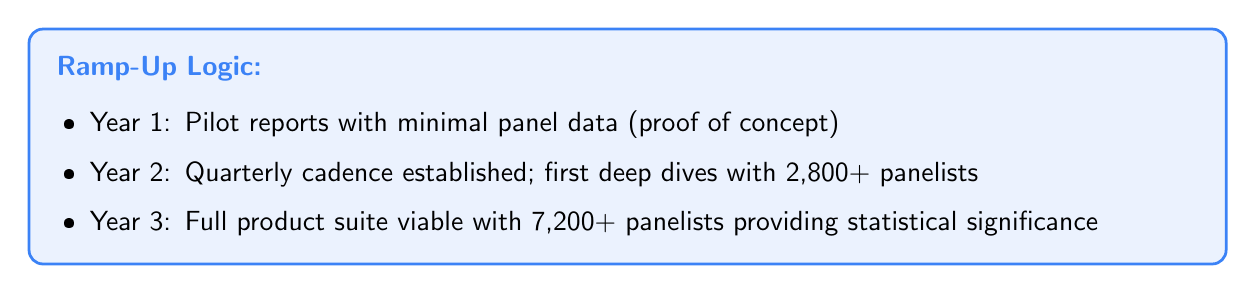
\begin{tikzpicture}
    \node[fill=infoblue!10, draw=infoblue, line width=1pt, rounded corners=5pt,
          inner sep=10pt, text width=14.5cm, align=left] {
        \textcolor{infoblue}{\textbf{Ramp-Up Logic:}}
        \begin{itemize}[leftmargin=1.2em, itemsep=2pt]
            \item Year 1: Pilot reports with minimal panel data (proof of concept)
            \item Year 2: Quarterly cadence established; first deep dives with 2,800+ panelists
            \item Year 3: Full product suite viable with 7,200+ panelists providing statistical significance
        \end{itemize}
    };
\end{tikzpicture}
\end{center}

\newpage

% ============================================================================
% COMPREHENSIVE P&L STATEMENT
% ============================================================================
\section*{\textcolor{miloprimary}{Comprehensive P\&L Statement}}

\subsection*{\textcolor{milosecondary}{Annual Profit \& Loss (Conservative Projections)}}

\begin{center}
\renewcommand{\arraystretch}{1.5}
\begin{tabular}{>{\raggedright\arraybackslash}p{5.5cm} >{\centering\arraybackslash}p{2.8cm} >{\centering\arraybackslash}p{2.8cm} >{\centering\arraybackslash}p{2.8cm}}
\toprule
\rowcolor{miloprimary!15}
\textbf{Line Item} & \textbf{Year 1} & \textbf{Year 2} & \textbf{Year 3} \\
\midrule
\multicolumn{4}{l}{\textbf{\textcolor{miloprimary}{REVENUE}}} \\
\rowcolor{appstoreblue!5}
\quad App Store (B2C) & \$105K & \$423K & \$951K \\
\rowcolor{datapurple!5}
\quad Dataset Monetization (B2B) & \$28K & \$225K & \$637K \\
\rowcolor{analyticsteal!5}
\quad Analytics Reports & \$11K & \$72K & \$212K \\
\rowcolor{successgreen!10}
\textbf{Total Revenue} & \textbf{\$144K} & \textbf{\$720K} & \textbf{\$1,800K} \\
\midrule
\multicolumn{4}{l}{\textbf{\textcolor{miloprimary}{COST OF REVENUE (Variable)}}} \\
\rowcolor{lightbg}
\quad Veryfi OCR Processing & \$26K & \$83K & \$179K \\
\quad Gemini API & \$1K & \$3K & \$6K \\
\rowcolor{lightbg}
\quad Firebase/Storage & \$1K & \$4K & \$8K \\
\quad Payment Processing (Apple 15\%) & \$8K & \$26K & \$39K \\
\rowcolor{warningorange!8}
\textbf{Total Variable Costs} & \textbf{\$36K} & \textbf{\$116K} & \textbf{\$232K} \\
\midrule
\rowcolor{successgreen!8}
\textbf{GROSS PROFIT} & \textbf{\$108K} & \textbf{\$604K} & \textbf{\$1,568K} \\
\rowcolor{successgreen!15}
\textbf{Gross Margin} & \textbf{75\%} & \textbf{84\%} & \textbf{87\%} \\
\midrule
\multicolumn{4}{l}{\textbf{\textcolor{miloprimary}{OPERATING EXPENSES (Fixed)}}} \\
\rowcolor{lightbg}
\quad Engineering \& Product & \$100K & \$180K & \$300K \\
\quad Sales \& Marketing & \$75K & \$150K & \$200K \\
\rowcolor{lightbg}
\quad B2B Sales Team & \$25K & \$80K & \$120K \\
\quad Legal \& Compliance (GDPR) & \$40K & \$60K & \$75K \\
\rowcolor{lightbg}
\quad Customer Support & \$10K & \$25K & \$40K \\
\quad Infrastructure (non-API) & \$10K & \$15K & \$20K \\
\rowcolor{miloprimary!8}
\textbf{Total Operating Expenses} & \textbf{\$260K} & \textbf{\$510K} & \textbf{\$755K} \\
\midrule
\rowcolor{dangerred!10}
\textbf{OPERATING PROFIT/(LOSS)} & \textbf{(\$152K)} & \textbf{\$94K} & \textbf{\$813K} \\
\rowcolor{miloprimary!15}
\textbf{Operating Margin} & \textbf{-106\%} & \textbf{13\%} & \textbf{45\%} \\
\bottomrule
\end{tabular}
\end{center}

\vspace{0.5cm}

\begin{center}
\alertbox{successgreen}{Strong Path to Profitability}{
\begin{itemize}[leftmargin=1.5em, itemsep=4pt]
    \item \textbf{Year 1:} Investment phase with \$152K operating loss (manageable with seed funding)
    \item \textbf{Year 2:} Break-even achieved with \$94K operating profit (13\% margin)
    \item \textbf{Year 3:} Strong profitability with \$813K operating profit (45\% margin)
    \item \textbf{Gross margins} improve from 75\% to 87\% as B2B mix increases (higher-margin revenue)
\end{itemize}
}
\end{center}

\newpage

% ============================================================================
% MARGIN ANALYSIS
% ============================================================================
\section*{\textcolor{miloprimary}{Margin Analysis by Revenue Stream}}

\subsection*{\textcolor{milosecondary}{Contribution Margin by Pillar}}

\begin{center}
\renewcommand{\arraystretch}{1.6}
\begin{tabular}{>{\raggedright\arraybackslash}p{3.5cm} >{\centering\arraybackslash}p{2cm} >{\centering\arraybackslash}p{2.2cm} >{\centering\arraybackslash}p{2.2cm} >{\centering\arraybackslash}p{2.2cm} >{\centering\arraybackslash}p{2cm}}
\toprule
\rowcolor{miloprimary!15}
\textbf{Revenue Stream} & \textbf{Y3 Rev} & \textbf{Variable Cost} & \textbf{Contribution} & \textbf{CM \%} & \textbf{CM/User} \\
\midrule
\rowcolor{appstoreblue!8}
\textcolor{appstoreblue}{\textbf{App Store}} & \$951K & \$357K & \$594K & 62\% & \$33/user \\
\rowcolor{datapurple!8}
\textcolor{datapurple}{\textbf{Datasets}} & \$637K & \$140K & \$497K & 78\% & \$69/panelist \\
\rowcolor{analyticsteal!8}
\textcolor{analyticsteal}{\textbf{Analytics}} & \$212K & \$32K & \$180K & 85\% & N/A \\
\midrule
\rowcolor{successgreen!10}
\textbf{Total} & \textbf{\$1,800K} & \textbf{\$529K*} & \textbf{\$1,271K} & \textbf{71\%} & -- \\
\bottomrule
\end{tabular}
\end{center}

\vspace{0.2cm}
{\small *Note: Variable costs include allocated OCR, API, and processing costs. Total differs from P\&L due to allocation methodology.}

\vspace{0.5cm}

\subsection*{\textcolor{milosecondary}{Why B2B Margins Are Higher}}

\begin{center}
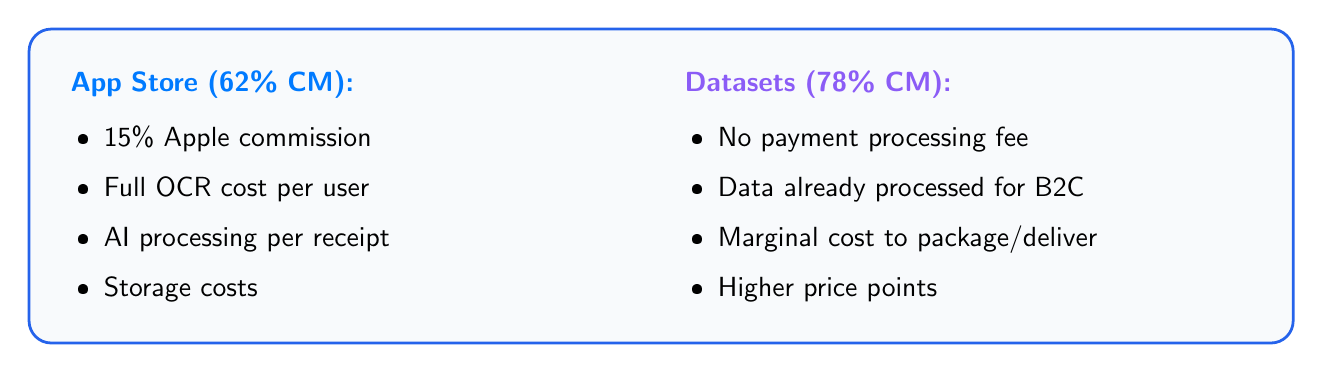
\begin{tikzpicture}
    \node[fill=lightbg, draw=miloprimary, line width=1pt, rounded corners=8pt,
          inner sep=15pt, text width=15cm, align=left] {
        \begin{minipage}[t]{0.48\textwidth}
            \textcolor{appstoreblue}{\textbf{App Store (62\% CM):}}
            \begin{itemize}[leftmargin=1.2em, itemsep=2pt]
                \item 15\% Apple commission
                \item Full OCR cost per user
                \item AI processing per receipt
                \item Storage costs
            \end{itemize}
        \end{minipage}
        \hfill
        \begin{minipage}[t]{0.48\textwidth}
            \textcolor{datapurple}{\textbf{Datasets (78\% CM):}}
            \begin{itemize}[leftmargin=1.2em, itemsep=2pt]
                \item No payment processing fee
                \item Data already processed for B2C
                \item Marginal cost to package/deliver
                \item Higher price points
            \end{itemize}
        \end{minipage}
    };
\end{tikzpicture}
\end{center}

\vspace{0.5cm}

\subsection*{\textcolor{milosecondary}{Gross Margin Trend}}

\begin{center}
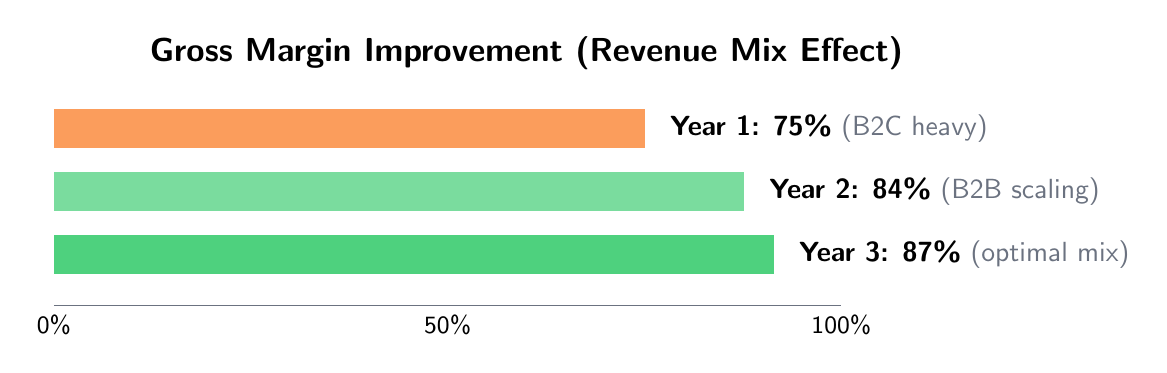
\begin{tikzpicture}
    % Title
    \node[align=center] at (0,4) {\textbf{\large Gross Margin Improvement (Revenue Mix Effect)}};

    % Year 1 bar
    \fill[warningorange!70] (-6,2.8) rectangle (1.5,3.3);
    \node[right] at (1.7,3.05) {\textbf{Year 1: 75\%} \textcolor{freegray}{(B2C heavy)}};

    % Year 2 bar
    \fill[successgreen!60] (-6,2) rectangle (2.76,2.5);
    \node[right] at (2.96,2.25) {\textbf{Year 2: 84\%} \textcolor{freegray}{(B2B scaling)}};

    % Year 3 bar
    \fill[successgreen!80] (-6,1.2) rectangle (3.14,1.7);
    \node[right] at (3.34,1.45) {\textbf{Year 3: 87\%} \textcolor{freegray}{(optimal mix)}};

    % Scale
    \draw[line width=0.5pt, freegray] (-6,0.8) -- (4,0.8);
    \node[below] at (-6,0.8) {\small 0\%};
    \node[below] at (-1,0.8) {\small 50\%};
    \node[below] at (4,0.8) {\small 100\%};
\end{tikzpicture}
\end{center}

\vspace{0.3cm}

\begin{center}
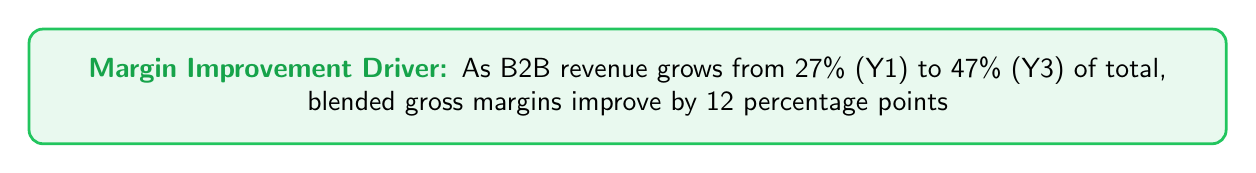
\begin{tikzpicture}
    \node[fill=successgreen!10, draw=successgreen, line width=1pt, rounded corners=5pt,
          inner sep=10pt, text width=14.5cm, align=center] {
        \textcolor{darkgreen}{\textbf{Margin Improvement Driver:}} As B2B revenue grows from 27\% (Y1) to 47\% (Y3) of total,\\blended gross margins improve by 12 percentage points
    };
\end{tikzpicture}
\end{center}

\newpage

% ============================================================================
% UNIT ECONOMICS
% ============================================================================
\section*{\textcolor{miloprimary}{Unit Economics Analysis}}

\subsection*{\textcolor{milosecondary}{Customer Acquisition Economics}}

\begin{center}
\renewcommand{\arraystretch}{1.6}
\begin{tabular}{>{\raggedright\arraybackslash}p{5cm} >{\centering\arraybackslash}p{3cm} >{\centering\arraybackslash}p{3cm} >{\centering\arraybackslash}p{3cm}}
\toprule
\rowcolor{miloprimary!15}
\textbf{Metric} & \textbf{Year 1} & \textbf{Year 2} & \textbf{Year 3} \\
\midrule
Marketing Spend & \$75K & \$150K & \$200K \\
\rowcolor{lightbg}
New Paid Customers & 2,000 & 6,500 & 11,000 \\
\textbf{Customer Acquisition Cost (CAC)} & \textbf{\$37.50} & \textbf{\$23.08} & \textbf{\$18.18} \\
\rowcolor{lightbg}
Trial Users per \$ Spent & 0.20 & 0.32 & 0.45 \\
\bottomrule
\end{tabular}
\end{center}

\vspace{0.3cm}

\begin{center}

\begin{tikzpicture}
    \node[fill=successgreen!10, draw=successgreen, line width=1pt, rounded corners=5pt,
          inner sep=10pt, text width=14.5cm, align=center] {
        \textcolor{darkgreen}{\textbf{CAC Efficiency:}} Acquisition costs decrease 52\% from Year 1 to Year 3\\as brand awareness builds and word-of-mouth contributes to growth
    };
\end{tikzpicture}
\end{center}

\vspace{0.5cm}

\subsection*{\textcolor{milosecondary}{Customer Lifetime Value (LTV)}}

\begin{center}
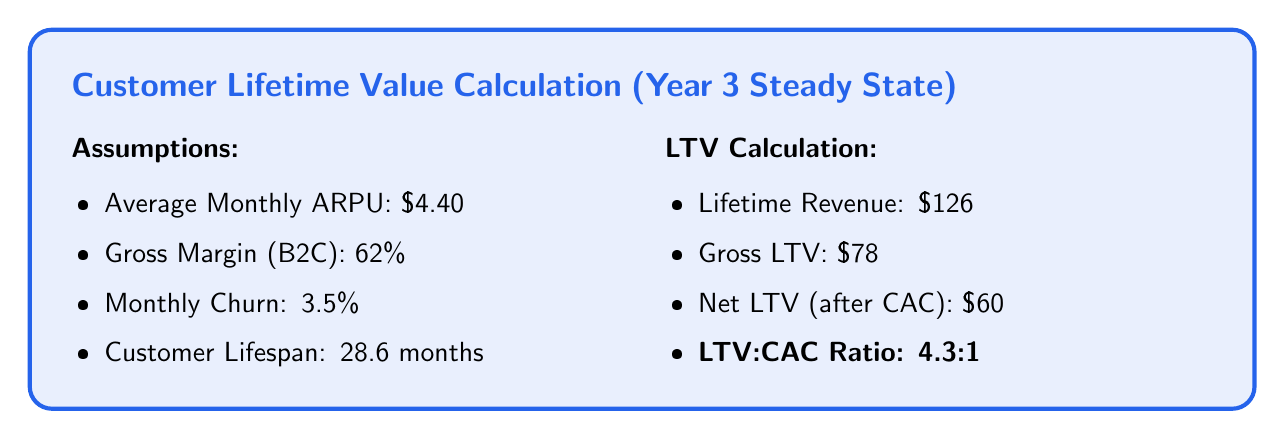
\begin{tikzpicture}
    \node[fill=miloprimary!10, draw=miloprimary, line width=1.5pt, rounded corners=8pt,
          inner sep=15pt, text width=14.5cm, align=left] {
        \textcolor{miloprimary}{\textbf{\large Customer Lifetime Value Calculation (Year 3 Steady State)}}\\[10pt]
        \begin{minipage}[t]{0.48\textwidth}
            \textbf{Assumptions:}
            \begin{itemize}[leftmargin=1.2em, itemsep=2pt]
                \item Average Monthly ARPU: \$4.40
                \item Gross Margin (B2C): 62\%
                \item Monthly Churn: 3.5\%
                \item Customer Lifespan: 28.6 months
            \end{itemize}
        \end{minipage}
        \hfill
        \begin{minipage}[t]{0.48\textwidth}
            \textbf{LTV Calculation:}
            \begin{itemize}[leftmargin=1.2em, itemsep=2pt]
                \item Lifetime Revenue: \$126
                \item Gross LTV: \$78
                \item Net LTV (after CAC): \$60
                \item \textbf{LTV:CAC Ratio: 4.3:1}
            \end{itemize}
        \end{minipage}
    };
\end{tikzpicture}
\end{center}

\vspace{0.5cm}

\subsection*{\textcolor{milosecondary}{LTV:CAC Ratio by Tier}}

\begin{center}
\renewcommand{\arraystretch}{1.5}
\begin{tabular}{>{\raggedright\arraybackslash}p{3cm} >{\centering\arraybackslash}p{2cm} >{\centering\arraybackslash}p{2.5cm} >{\centering\arraybackslash}p{2.5cm} >{\centering\arraybackslash}p{2cm} >{\centering\arraybackslash}p{2cm}}
\toprule
\rowcolor{miloprimary!15}
\textbf{Tier} & \textbf{Price} & \textbf{Lifetime Rev} & \textbf{Gross LTV} & \textbf{CAC} & \textbf{LTV:CAC} \\
\midrule
\rowcolor{bronzecolor!8}
\textcolor{bronzecolor}{\textbf{Bronze}} & \$2/mo & \$57 & \$35 & \$18 & 1.9:1 \\
\rowcolor{silvercolor!8}
\textcolor{silvercolor}{\textbf{Silver}} & \$4/mo & \$114 & \$71 & \$18 & 3.9:1 \\
\rowcolor{goldcolor!8}
\textcolor{goldcolor}{\textbf{Gold}} & \$6/mo & \$172 & \$107 & \$18 & 5.9:1 \\
\rowcolor{platinumcolor!8}
\textcolor{platinumcolor}{\textbf{Platinum}} & \$10/mo & \$286 & \$177 & \$18 & 9.8:1 \\
\midrule
\rowcolor{successgreen!10}
\textbf{Blended Average} & \$4.40/mo & \$126 & \$78 & \$18 & \textbf{4.3:1} \\
\bottomrule
\end{tabular}
\end{center}

\vspace{0.3cm}

\begin{center}
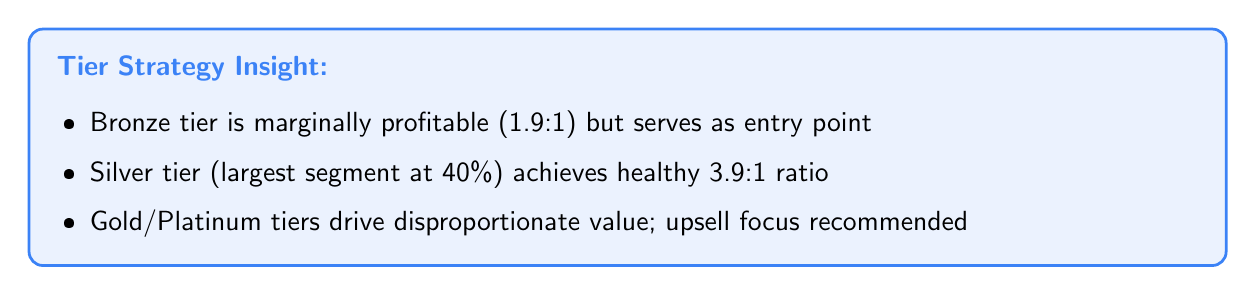
\begin{tikzpicture}
    \node[fill=infoblue!10, draw=infoblue, line width=1pt, rounded corners=5pt,
          inner sep=10pt, text width=14.5cm, align=left] {
        \textcolor{infoblue}{\textbf{Tier Strategy Insight:}}
        \begin{itemize}[leftmargin=1.2em, itemsep=2pt]
            \item Bronze tier is marginally profitable (1.9:1) but serves as entry point
            \item Silver tier (largest segment at 40\%) achieves healthy 3.9:1 ratio
            \item Gold/Platinum tiers drive disproportionate value; upsell focus recommended
        \end{itemize}
    };
\end{tikzpicture}
\end{center}

\newpage

% ============================================================================
% BREAK-EVEN ANALYSIS
% ============================================================================
\section*{\textcolor{miloprimary}{Break-Even Analysis}}

\subsection*{\textcolor{milosecondary}{Monthly Break-Even Calculation}}

\begin{center}
\renewcommand{\arraystretch}{1.5}
\begin{tabular}{>{\raggedright\arraybackslash}p{6cm} >{\centering\arraybackslash}p{4cm} >{\centering\arraybackslash}p{4cm}}
\toprule
\rowcolor{miloprimary!15}
\textbf{Variable} & \textbf{Year 1} & \textbf{Year 3 (Steady State)} \\
\midrule
Monthly Fixed Costs & \$21,667 & \$62,917 \\
\rowcolor{lightbg}
Blended Contribution Margin & 75\% & 87\% \\
\textbf{Break-Even Monthly Revenue} & \textbf{\$28,889} & \textbf{\$72,318} \\
\rowcolor{lightbg}
\textbf{Break-Even Paid Users} & \textbf{\~{}5,500} & \textbf{\~{}11,000} \\
\bottomrule
\end{tabular}
\end{center}

\vspace{0.5cm}

\subsection*{\textcolor{milosecondary}{Break-Even Timeline}}

\begin{center}
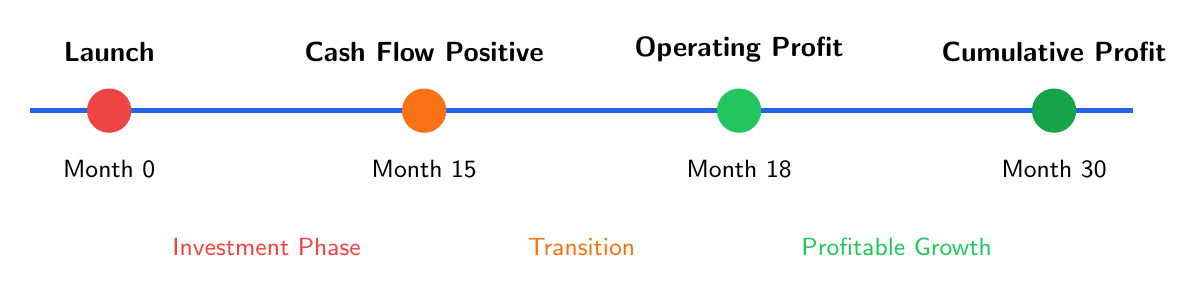
\begin{tikzpicture}
    % Timeline
    \draw[line width=2pt, miloprimary] (-7,0) -- (7,0);

    % Markers
    \fill[dangerred] (-6,0) circle (8pt);
    \node[above] at (-6,0.5) {\textbf{Launch}};
    \node[below] at (-6,-0.5) {\small Month 0};

    \fill[warningorange] (-2,0) circle (8pt);
    \node[above] at (-2,0.5) {\textbf{Cash Flow Positive}};
    \node[below] at (-2,-0.5) {\small Month 15};

    \fill[successgreen] (2,0) circle (8pt);
    \node[above] at (2,0.5) {\textbf{Operating Profit}};
    \node[below] at (2,-0.5) {\small Month 18};

    \fill[darkgreen] (6,0) circle (8pt);
    \node[above] at (6,0.5) {\textbf{Cumulative Profit}};
    \node[below] at (6,-0.5) {\small Month 30};

    % Phase labels
    \node[below] at (-4,-1.5) {\textcolor{dangerred}{\small Investment Phase}};
    \node[below] at (0,-1.5) {\textcolor{warningorange}{\small Transition}};
    \node[below] at (4,-1.5) {\textcolor{successgreen}{\small Profitable Growth}};
\end{tikzpicture}
\end{center}

\vspace{0.5cm}

\subsection*{\textcolor{milosecondary}{Scenario Analysis: Break-Even Timing}}

\begin{center}
\renewcommand{\arraystretch}{1.5}
\begin{tabular}{>{\raggedright\arraybackslash}p{3.5cm} >{\centering\arraybackslash}p{2.5cm} >{\centering\arraybackslash}p{2.5cm} >{\centering\arraybackslash}p{2.5cm} >{\centering\arraybackslash}p{2.5cm}}
\toprule
\rowcolor{miloprimary!15}
\textbf{Scenario} & \textbf{Monthly Rev} & \textbf{Paid Users} & \textbf{Break-Even} & \textbf{Probability} \\
\midrule
\rowcolor{dangerred!10}
\textbf{Bear Case} & \$40K & 7,500 & Month 24 & 20\% \\
\rowcolor{lightbg}
\textbf{Base Case} & \$60K & 11,000 & Month 18 & 60\% \\
\rowcolor{successgreen!10}
\textbf{Bull Case} & \$85K & 15,000 & Month 14 & 20\% \\
\bottomrule
\end{tabular}
\end{center}

\vspace{0.5cm}

\begin{center}
\alertbox{warningorange}{Funding Runway Requirement}{
\begin{itemize}[leftmargin=1.5em, itemsep=4pt]
    \item \textbf{Year 1 Operating Loss:} \$152K
    \item \textbf{Working Capital Buffer:} \$50K (3 months expenses)
    \item \textbf{Minimum Funding Required:} \$200K seed round
    \item \textbf{Recommended Funding:} \$300K (provides 18-month runway to profitability)
\end{itemize}
}
\end{center}

\newpage

% ============================================================================
% CASH FLOW ANALYSIS
% ============================================================================
\section*{\textcolor{miloprimary}{Cash Flow Analysis}}

\subsection*{\textcolor{milosecondary}{Monthly Cash Position (Year 1)}}

\begin{center}
\renewcommand{\arraystretch}{1.5}
\begin{tabular}{>{\centering\arraybackslash}p{1.8cm} >{\centering\arraybackslash}p{2cm} >{\centering\arraybackslash}p{2cm} >{\centering\arraybackslash}p{2cm} >{\centering\arraybackslash}p{2cm} >{\centering\arraybackslash}p{2.5cm}}
\toprule
\rowcolor{miloprimary!15}
\textbf{Month} & \textbf{Revenue} & \textbf{Var. Costs} & \textbf{Fixed Costs} & \textbf{Net Cash} & \textbf{Cumulative} \\
\midrule
M1 & \$3K & \$1K & \$22K & (\$20K) & (\$20K) \\
\rowcolor{lightbg}
M3 & \$7K & \$2K & \$22K & (\$17K) & (\$54K) \\
M6 & \$14K & \$3K & \$22K & (\$11K) & (\$87K) \\
\rowcolor{lightbg}
M9 & \$22K & \$5K & \$22K & (\$5K) & (\$112K) \\
M12 & \$32K & \$8K & \$22K & \$2K & (\$132K) \\
\bottomrule
\end{tabular}
\end{center}

\vspace{0.5cm}

\subsection*{\textcolor{milosecondary}{Annual Cash Flow Summary}}

\begin{center}
\renewcommand{\arraystretch}{1.5}
\begin{tabular}{>{\raggedright\arraybackslash}p{5cm} >{\centering\arraybackslash}p{3cm} >{\centering\arraybackslash}p{3cm} >{\centering\arraybackslash}p{3cm}}
\toprule
\rowcolor{miloprimary!15}
\textbf{Cash Flow Item} & \textbf{Year 1} & \textbf{Year 2} & \textbf{Year 3} \\
\midrule
Operating Cash Flow & (\$152K) & \$94K & \$813K \\
\rowcolor{lightbg}
Beginning Cash (with \$300K funding) & \$300K & \$148K & \$242K \\
\textbf{Ending Cash Position} & \textbf{\$148K} & \textbf{\$242K} & \textbf{\$1,055K} \\
\rowcolor{successgreen!10}
\textbf{Months Runway} & 9 months & 5 months & 17 months \\
\bottomrule
\end{tabular}
\end{center}

\vspace{0.5cm}

\begin{center}
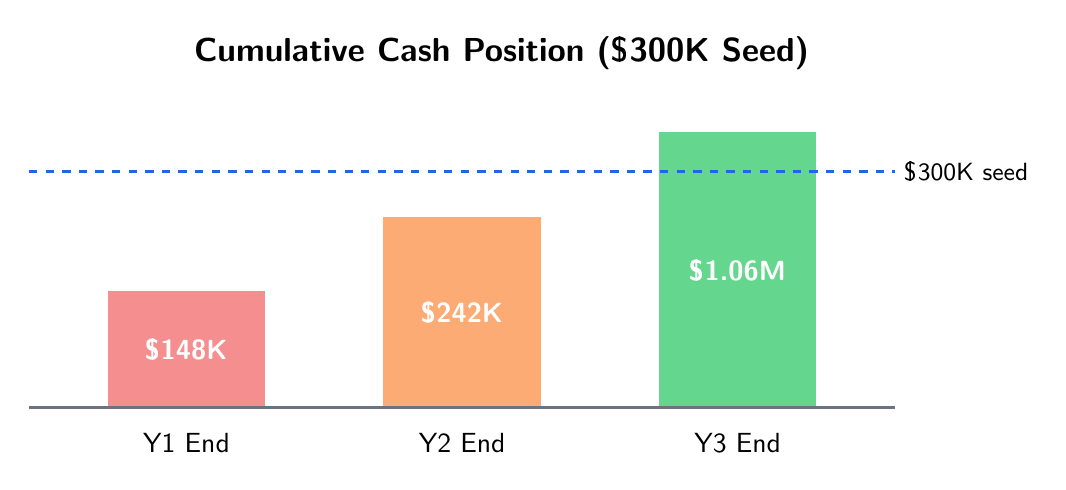
\begin{tikzpicture}
    % Title
    \node[align=center] at (0,4.5) {\textbf{\large Cumulative Cash Position (\$300K Seed)}};

    % Bars
    \fill[dangerred!60] (-5,0) rectangle (-3,1.48);
    \node at (-4,0.74) {\textcolor{white}{\textbf{\$148K}}};
    \node[below] at (-4,-0.2) {Y1 End};

    \fill[warningorange!60] (-1.5,0) rectangle (0.5,2.42);
    \node at (-0.5,1.21) {\textcolor{white}{\textbf{\$242K}}};
    \node[below] at (-0.5,-0.2) {Y2 End};

    \fill[successgreen!70] (2,0) rectangle (4,3.5);
    \node at (3,1.75) {\textcolor{white}{\textbf{\$1.06M}}};
    \node[below] at (3,-0.2) {Y3 End};

    % Baseline
    \draw[line width=1pt, freegray] (-6,0) -- (5,0);

    % Reference line for seed
    \draw[dashed, line width=1pt, miloprimary] (-6,3) -- (5,3);
    \node[right] at (5,3) {\small \$300K seed};
\end{tikzpicture}
\end{center}

\newpage

% ============================================================================
% SENSITIVITY ANALYSIS
% ============================================================================
\section*{\textcolor{miloprimary}{Sensitivity Analysis}}

\subsection*{\textcolor{milosecondary}{Key Variable Impact on Year 3 Operating Profit}}

\begin{center}
\renewcommand{\arraystretch}{1.5}
\begin{tabular}{>{\raggedright\arraybackslash}p{4cm} >{\centering\arraybackslash}p{2.2cm} >{\centering\arraybackslash}p{2.2cm} >{\centering\arraybackslash}p{2.2cm} >{\centering\arraybackslash}p{2.2cm}}
\toprule
\rowcolor{miloprimary!15}
\textbf{Variable} & \textbf{-20\%} & \textbf{Base Case} & \textbf{+20\%} & \textbf{Impact} \\
\midrule
\rowcolor{dangerred!10}
Trial Conversion Rate & \$493K & \$813K & \$1,133K & \cellcolor{dangerred!20}\textbf{HIGH} \\
\rowcolor{dangerred!10}
Data Consent Rate & \$685K & \$813K & \$941K & \cellcolor{dangerred!20}\textbf{HIGH} \\
\rowcolor{warningorange!10}
User Churn Rate & \$973K & \$813K & \$653K & \cellcolor{warningorange!20}MEDIUM \\
\rowcolor{warningorange!10}
Veryfi OCR Costs & \$849K & \$813K & \$777K & \cellcolor{warningorange!20}MEDIUM \\
\rowcolor{successgreen!10}
Engineering Costs & \$873K & \$813K & \$753K & \cellcolor{successgreen!20}LOW \\
\bottomrule
\end{tabular}
\end{center}

\vspace{0.5cm}

\subsection*{\textcolor{milosecondary}{Critical Success Factors}}

\begin{center}
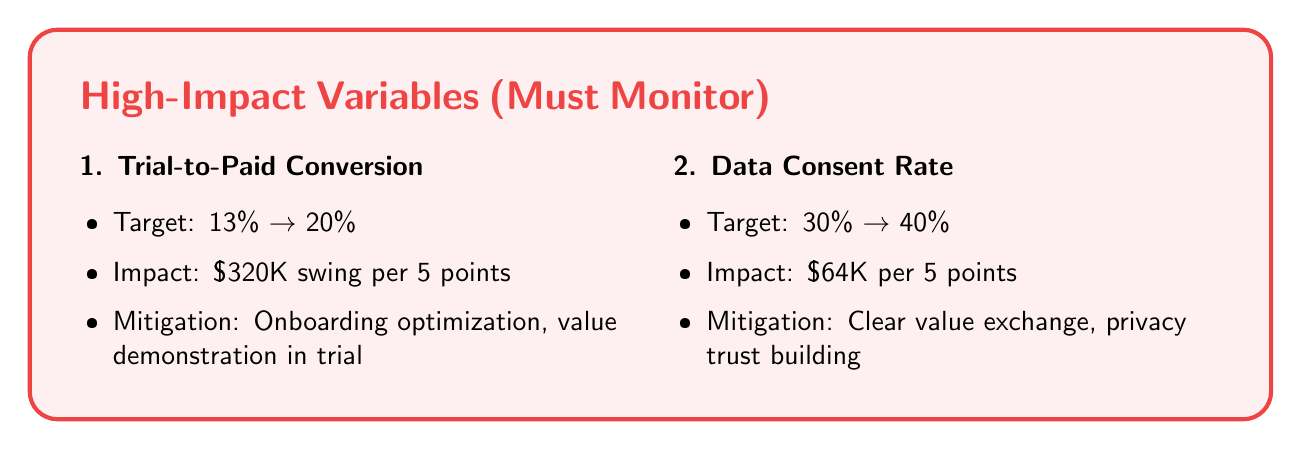
\begin{tikzpicture}
    \node[fill=dangerred!8, draw=dangerred, line width=1.5pt, rounded corners=10pt,
          inner sep=18pt, text width=14.5cm, align=left] {
        {\Large\textcolor{dangerred}{\textbf{High-Impact Variables (Must Monitor)}}}\\[12pt]
        \begin{minipage}[t]{0.48\textwidth}
            \textbf{1. Trial-to-Paid Conversion}
            \begin{itemize}[leftmargin=1.2em, itemsep=2pt]
                \item Target: 13\% $\rightarrow$ 20\%
                \item Impact: \$320K swing per 5 points
                \item Mitigation: Onboarding optimization, value demonstration in trial
            \end{itemize}
        \end{minipage}
        \hfill
        \begin{minipage}[t]{0.48\textwidth}
            \textbf{2. Data Consent Rate}
            \begin{itemize}[leftmargin=1.2em, itemsep=2pt]
                \item Target: 30\% $\rightarrow$ 40\%
                \item Impact: \$64K per 5 points
                \item Mitigation: Clear value exchange, privacy trust building
            \end{itemize}
        \end{minipage}
    };
\end{tikzpicture}
\end{center}

\vspace{0.5cm}

\subsection*{\textcolor{milosecondary}{Scenario Analysis: 3-Year Operating Profit}}

\begin{center}
\renewcommand{\arraystretch}{1.5}
\begin{tabular}{>{\raggedright\arraybackslash}p{3.5cm} >{\centering\arraybackslash}p{2.2cm} >{\centering\arraybackslash}p{2.2cm} >{\centering\arraybackslash}p{2.2cm} >{\centering\arraybackslash}p{2.2cm} >{\centering\arraybackslash}p{2cm}}
\toprule
\rowcolor{miloprimary!15}
\textbf{Scenario} & \textbf{Year 1} & \textbf{Year 2} & \textbf{Year 3} & \textbf{3-Yr Total} & \textbf{Prob.} \\
\midrule
\rowcolor{dangerred!10}
\textbf{Bear Case} & (\$190K) & (\$50K) & \$350K & \$110K & 20\% \\
\rowcolor{lightbg}
\textbf{Base Case} & (\$152K) & \$94K & \$813K & \$755K & 60\% \\
\rowcolor{successgreen!10}
\textbf{Bull Case} & (\$100K) & \$250K & \$1,300K & \$1,450K & 20\% \\
\midrule
\rowcolor{miloprimary!10}
\textbf{Expected Value} & (\$146K) & \$87K & \$761K & \textbf{\$702K} & -- \\
\bottomrule
\end{tabular}
\end{center}

\newpage

% ============================================================================
% RISK ANALYSIS
% ============================================================================
\section*{\textcolor{miloprimary}{Risk Analysis \& Mitigation}}

\subsection*{\textcolor{milosecondary}{Revenue Risk Matrix}}

\begin{center}
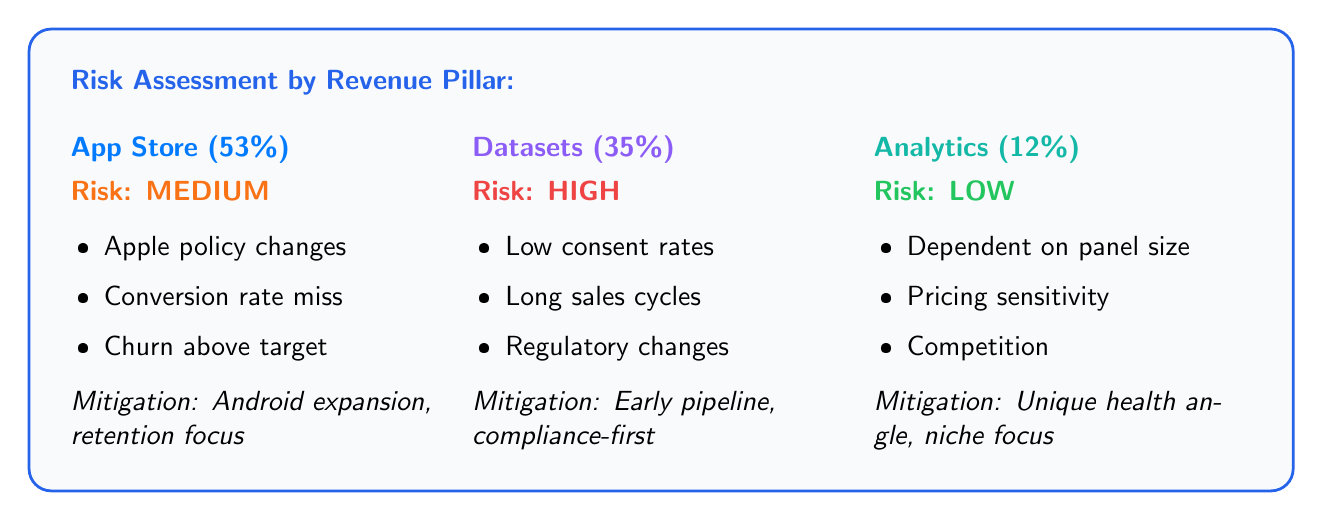
\begin{tikzpicture}
    \node[fill=lightbg, draw=miloprimary, line width=1pt, rounded corners=8pt,
          inner sep=15pt, text width=15cm, align=left] {
        \textcolor{miloprimary}{\textbf{Risk Assessment by Revenue Pillar:}}\\[12pt]
        \begin{minipage}[t]{0.32\textwidth}
            \textcolor{appstoreblue}{\textbf{App Store (53\%)}}\\[4pt]
            \textcolor{warningorange}{\textbf{Risk: MEDIUM}}
            \begin{itemize}[leftmargin=1.2em, itemsep=2pt]
                \item Apple policy changes
                \item Conversion rate miss
                \item Churn above target
            \end{itemize}
            \textit{Mitigation: Android expansion, retention focus}
        \end{minipage}
        \hfill
        \begin{minipage}[t]{0.32\textwidth}
            \textcolor{datapurple}{\textbf{Datasets (35\%)}}\\[4pt]
            \textcolor{dangerred}{\textbf{Risk: HIGH}}
            \begin{itemize}[leftmargin=1.2em, itemsep=2pt]
                \item Low consent rates
                \item Long sales cycles
                \item Regulatory changes
            \end{itemize}
            \textit{Mitigation: Early pipeline, compliance-first}
        \end{minipage}
        \hfill
        \begin{minipage}[t]{0.32\textwidth}
            \textcolor{analyticsteal}{\textbf{Analytics (12\%)}}\\[4pt]
            \textcolor{successgreen}{\textbf{Risk: LOW}}
            \begin{itemize}[leftmargin=1.2em, itemsep=2pt]
                \item Dependent on panel size
                \item Pricing sensitivity
                \item Competition
            \end{itemize}
            \textit{Mitigation: Unique health angle, niche focus}
        \end{minipage}
    };
\end{tikzpicture}
\end{center}

\vspace{0.5cm}

\subsection*{\textcolor{milosecondary}{Key Risks \& Mitigations}}

\begin{center}
\renewcommand{\arraystretch}{1.4}
\begin{tabular}{>{\raggedright\arraybackslash}p{3.5cm} >{\centering\arraybackslash}p{1.5cm} >{\centering\arraybackslash}p{1.5cm} >{\raggedright\arraybackslash}p{4cm} >{\raggedright\arraybackslash}p{3.5cm}}
\toprule
\rowcolor{miloprimary!15}
\textbf{Risk} & \textbf{Likelihood} & \textbf{Impact} & \textbf{Description} & \textbf{Mitigation} \\
\midrule
\rowcolor{dangerred!8}
Veryfi Dependency & Med & High & 77\% of variable costs & Volume contracts, backup OCR \\
\rowcolor{warningorange!8}
Low Data Consent & Med & High & Impacts 35\% of revenue & Value exchange, trust building \\
\rowcolor{warningorange!8}
Conversion Miss & Med & Med & Below 13\% trial conversion & Onboarding optimization \\
\rowcolor{lightbg}
Enterprise Sales Delay & High & Med & 6-12 month cycles & Early pipeline building \\
\rowcolor{successgreen!8}
Competition & Low & Med & New entrants & AI moat, health differentiator \\
\bottomrule
\end{tabular}
\end{center}

\vspace{0.5cm}

\begin{center}
\alertbox{infoblue}{Diversification Benefit}{
The three-pillar model provides natural hedging:
\begin{itemize}[leftmargin=1.5em, itemsep=3pt]
    \item If B2C underperforms, B2B provides stability (longer contracts, predictable revenue)
    \item If B2B sales slow, B2C subscription base continues growing
    \item Analytics revenue requires minimal incremental cost once panel is established
    \item No single revenue stream exceeds 55\% of total by Year 3
\end{itemize}
}
\end{center}

\newpage

% ============================================================================
% CONCLUSION
% ============================================================================
\section*{\textcolor{miloprimary}{Conclusion \& Key Takeaways}}

\begin{center}
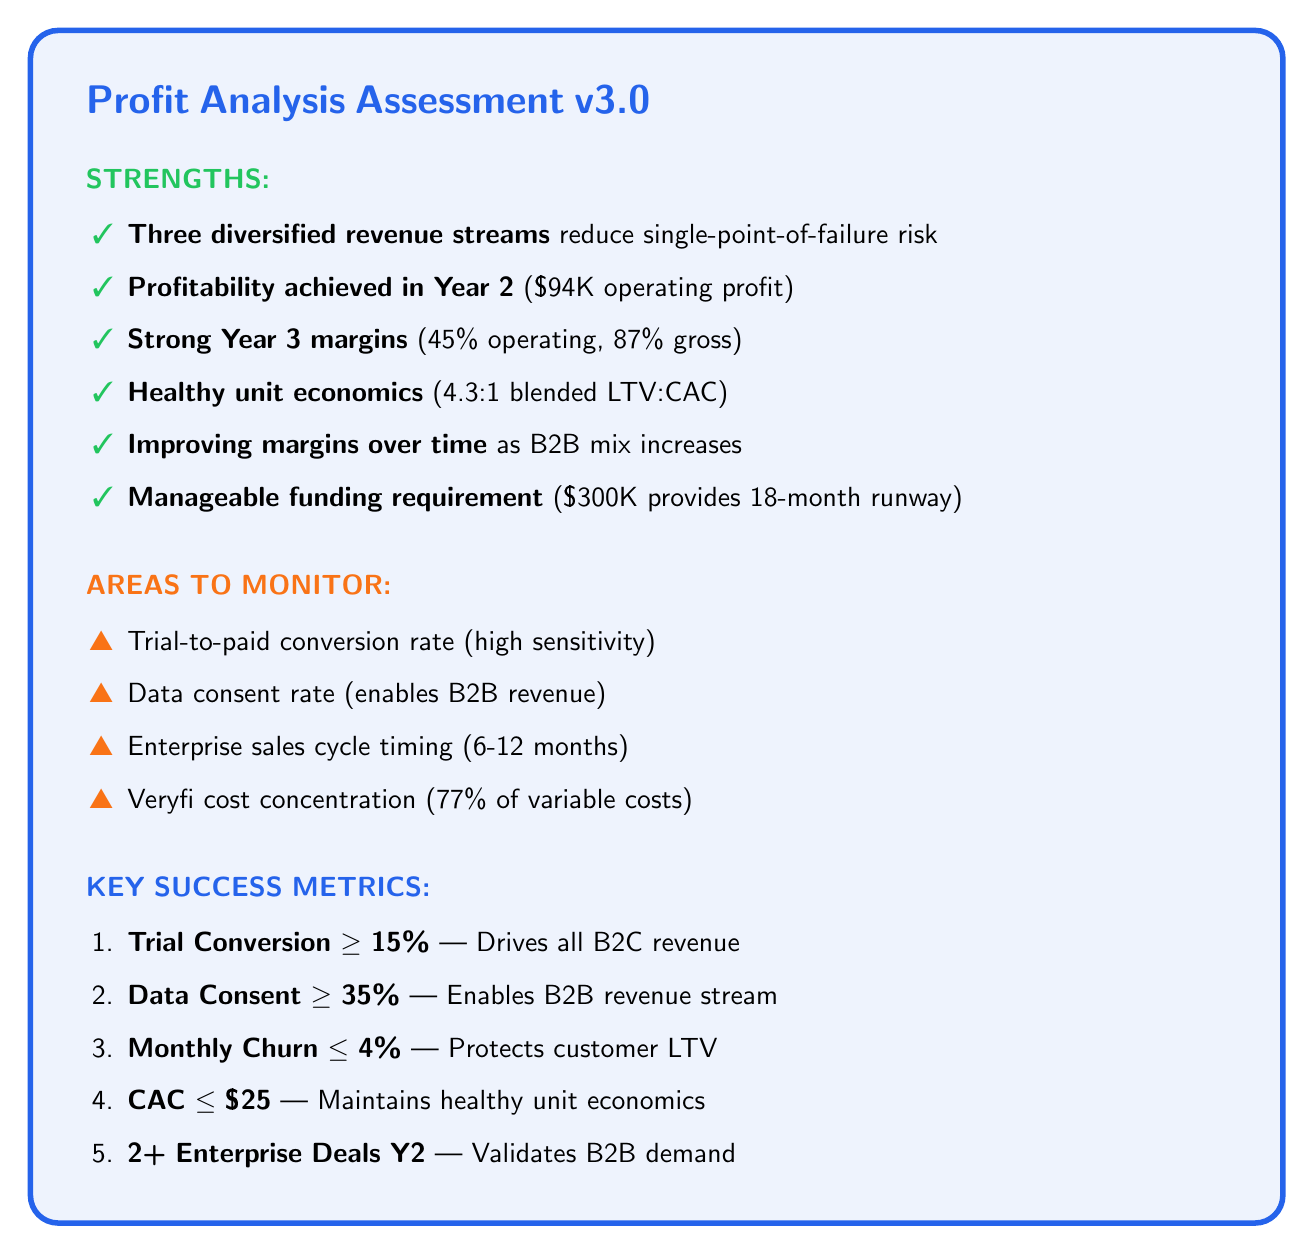
\begin{tikzpicture}
    \node[fill=miloprimary!8, draw=miloprimary, line width=2pt, rounded corners=10pt,
          inner sep=20pt, text width=14.5cm, align=left] {
        {\Large\textcolor{miloprimary}{\textbf{Profit Analysis Assessment v3.0}}}\\[15pt]

        \textcolor{successgreen}{\textbf{STRENGTHS:}}
        \begin{itemize}[leftmargin=1.5em, itemsep=3pt]
            \item[\cmark] \textbf{Three diversified revenue streams} reduce single-point-of-failure risk
            \item[\cmark] \textbf{Profitability achieved in Year 2} (\$94K operating profit)
            \item[\cmark] \textbf{Strong Year 3 margins} (45\% operating, 87\% gross)
            \item[\cmark] \textbf{Healthy unit economics} (4.3:1 blended LTV:CAC)
            \item[\cmark] \textbf{Improving margins over time} as B2B mix increases
            \item[\cmark] \textbf{Manageable funding requirement} (\$300K provides 18-month runway)
        \end{itemize}

        \vspace{12pt}
        \textcolor{warningorange}{\textbf{AREAS TO MONITOR:}}
        \begin{itemize}[leftmargin=1.5em, itemsep=3pt]
            \item[\wmark] Trial-to-paid conversion rate (high sensitivity)
            \item[\wmark] Data consent rate (enables B2B revenue)
            \item[\wmark] Enterprise sales cycle timing (6-12 months)
            \item[\wmark] Veryfi cost concentration (77\% of variable costs)
        \end{itemize}

        \vspace{12pt}
        \textcolor{miloprimary}{\textbf{KEY SUCCESS METRICS:}}
        \begin{itemize}[leftmargin=1.5em, itemsep=3pt]
            \item[1.] \textbf{Trial Conversion $\geq$ 15\%} --- Drives all B2C revenue
            \item[2.] \textbf{Data Consent $\geq$ 35\%} --- Enables B2B revenue stream
            \item[3.] \textbf{Monthly Churn $\leq$ 4\%} --- Protects customer LTV
            \item[4.] \textbf{CAC $\leq$ \$25} --- Maintains healthy unit economics
            \item[5.] \textbf{2+ Enterprise Deals Y2} --- Validates B2B demand
        \end{itemize}
    };
\end{tikzpicture}
\end{center}

\vspace{0.8cm}

% Summary Statistics
\begin{center}
    \statbox{dangerred}{Y1 Loss}{(\$152K)}
    \hspace{0.3cm}
    \statbox{successgreen}{Y2 Profit}{\$94K}
    \hspace{0.3cm}
    \statbox{darkgreen}{Y3 Profit}{\$813K}
    \hspace{0.3cm}
    \statbox{miloprimary}{3-Yr Total}{\$755K}
\end{center}

\vspace{1cm}

% Footer
\begin{center}
    \textcolor{freegray}{\rule{14cm}{0.5pt}}\\[0.4cm]
    \textcolor{freegray}{\small DeepmAInd B.V. | Confidential | Version 3.0 | January 2026}\\[0.2cm]
    \textcolor{freegray}{\scriptsize Based on v3.1 Cost Analysis | Conservative projections with realistic growth assumptions}
\end{center}

\end{document}
